%
% File acl2017.tex
%
%% Based on the style files for ACL-2015, with some improvements
%%  taken from the NAACL-2016 style
%% Based on the style files for ACL-2014, which were, in turn,
%% based on ACL-2013, ACL-2012, ACL-2011, ACL-2010, ACL-IJCNLP-2009,
%% EACL-2009, IJCNLP-2008...
%% Based on the style files for EACL 2006 by 
%%e.agirre@ehu.es or Sergi.Balari@uab.es
%% and that of ACL 08 by Joakim Nivre and Noah Smith

\documentclass[11pt,a4paper]{article}
\usepackage[hyperref]{acl2017}
\usepackage{times}
\usepackage{booktabs}
\usepackage{bbold}
\usepackage{latexsym}
\usepackage{graphicx}
\usepackage{float}
\usepackage{color}
\usepackage{subcaption}
\usepackage{url}

%\usepackage[draft]{hyperref}

%\aclfinalcopy % Uncomment this line for the final submission
%\def\aclpaperid{***} %  Enter the acl Paper ID here

%\setlength\titlebox{5cm}
% You can expand the titlebox if you need extra space
% to show all the authors. Please do not make the titlebox
% smaller than 5cm (the original size); we will check this
% in the camera-ready version and ask you to change it back.

\newcommand\BibTeX{B{\sc ib}\TeX}

\title{Joint Sentence-Document Model for Manifesto Text Analysis}

\author{First Author \\
  Affiliation / Address line 1 \\
  Affiliation / Address line 2 \\
  Affiliation / Address line 3 \\
  {\tt email@domain} \\\And
  Second Author \\
  Affiliation / Address line 1 \\
  Affiliation / Address line 2 \\
  Affiliation / Address line 3 \\
  {\tt email@domain} \\}

\date{}

\newcommand{\argmin}{\arg\!\min}
\newcommand{\norm}[1]{\vert #1 \vert}

\begin{document}
\maketitle
\begin{abstract}
Political parties are essential institutions of democracy. Election programs (so-called manifestos) is a published verbal declaration of the intentions, motives, or views of the political party.\footnote{\url{https://en.wikipedia.org/wiki/Manifesto}} Political scientists use manifestos to understand sentence level policy relevant themes discussed and also quantify party's position on the left-right spectrum. Rather than handling the two tasks separately, we propose a joint sentence-document model for sentence level thematic classification and document level position quantification using manifestos in different languages. Inorder to handle text from multiple languages we exploit continuous neural embeddings for semantic text representation. We have empirically shown the effectiveness of proposed approach using manifestos from thirteen countries which are written in six different languages.
\end{abstract}

% Secondly, all the works use manually coded thematic category distribution at sentence level as features for document level quantification task. Whereas, in this work we evaluate the effectiveness of using text for quantification task.
\section{Introduction}

Language is the medium for politics and political conflict. During election campaigns, individual candidates and political parties articulate their policy positions through party platforms and manifestos. Elected representatives debate legislation and vote for bills. After laws are passed, bureaucrats solicit comments before they issue regulations. The public discuss and express their views through social media (Twitter, blogs, Facebook), and they also launch campaigns for the change they wish to see through online petitions.  News reports document the day-to-day affairs of regional and international issues, in a way it covers information from many other sources.  It is apparent that understanding text is needed to know what political actors are speaking or writing. Though political scientists have long recognized the need for using text as data, it has not been explored due the difficulty in handling large amounts of text --- since hiring coders to manually annotate all documents was the common approach used. With automated text analysis, use of text for political data analysis is getting increased attention among political scientists \cite{ruedin2013role, gentzkow2017text}.

%Countries debate their stand on key issues in the UN. They regularly express statements that signal their priorities and also describe their motivations for cross-country ties.
%\footnote{\url{https://manifestoproject.wzb.eu/coding_schemes/mp_v5}}
Among many actors, political parties are at the core of contemporary democratic systems. One of the widely used dataset by political scientists includes the Comparative
Manifesto Project (CMP) dataset, initiated by \cite{CMP}, that collects party election programs (so-called manifestos) from elections in many countries around the world. The goal of the project is to provide a large data collection to support political studies on electoral processes. A sub-part of the manifestos has been manually annotated at sentence-level with one of over fifty fine-grained political themes, divided into 7 coarse-grained topics (schema is given in Figure \ref{fig:CMP}). Each sentence is segmented if it discusses more than one topic and labeled. While manual annotations are very useful for political analyses, they come with two major drawbacks. First, it is very time-consuming and labor-intensive to manually annotate each sentence with the correct category from a complex annotation scheme. Secondly, coders' preferences towards particular categories might cause annotation inconsistencies and affect comparability between manifestos annotated by different coders \cite{coder}. \cite{verberne2014automatic} is one of the early works using manifesto text for automatic thematic classification, using a topic hierarchy defined by Dutch political experts. In \cite{zirn2016classifying} authors worked with CMP dataset to do coarse-level topic classification (defined by CMP). They used Markov Logic Networks (MLN) to model sentence adjacency topic smoothness constraint. Nonetheless, manually coded manifestos remain the crucial data source for studies in computational political science \cite{lowe2011scaling, nanni}. 

Other than the sentence level labels, the manifesto text also has document level signals 
which quantifies its position in the left-right spectrum --- rile, expert survey and voter survey scores \cite{slapin2008scaling}. Though sentence level classification and document level quantification tasks are inter-dependent, existing works handle them separately.  Whereas, we propose a joint sentence-document model to handle both the tasks together. We use quantification and regression inter-changeably in this document.

\section{Related Works}

The recent adoption of NLP methods had led to significant advances in the field of Computational Social Science \cite{lazer2009life} including political science \cite{grimmer2013text}. Some popular tasks addressed with political text include party position analysis \cite{biessmann2016automating};  political leaning categorization \cite{akoglu2014quantifying, zhou2011classifying}; stance classification \cite{sridhar2014collective}; identifying keywords, themes \& topics \cite{karan2016analysis, nallapati2004extraction, ding2011keyphrase}; emotion analysis \cite{rheault2016expressions} and sentiment analysis \cite{bakliwal2013sentiment}. These works use manifestos, political speech, news articles, floor debates and social media posts. 

With the advancement of computational resources, large scale comparative political text analysis has gained the attention of political scientists, where the objective is to analyze large amounts of data uniformly in order to make it comparable \cite{lucas2015computer}. For example, rather than analyzing the political manifesto of a particular party during an election, mining different manifestos across countries over time can provide deeper comparative insights on political change.

Existing classification models, except \cite{W17-2906}, utilize discrete representation of text (i.e., bag of words) and can thus exploit only monolingual data (i.e., train and predict same language instances). Hence, most of the works analyze manifesto text at country level. Recent work has shown the use of neural embeddings for multi-lingual manifesto text coarse-level topic classification (7 major categories) \cite{W17-2906}. In \cite{W17-2906} authors show that multi-lingual embeddings are more effective for cross-lingual coarse-level manifesto text topic classification using labeled data across languages. In this work, we focus on cross-lingual fine-grained thematic classification (57 categories in total), where we have labeled data across all the languages.

For document level quantification task, many works use label count aggregation of  manually annotated sentences as features \cite{lowe2011scaling, benoit2014putting} and other works use dictionary based supervised methods (wordscores), unsupervised factor analysis based techniques (wordfish) \cite{hjorth2015computers, 2017arXiv170704737B}. Since the latter techniques use discrete word representation, they cannot be used for multi-lingual setting. In \cite{EACL}, authors leverage neural embeddings for EU parliament speech text quantification task with two pivot texts for extreme left and right positions. They represent the documents using word embeddings averaged with TF-IDF scores as weights. Rather than handling sentence and document-level tasks separately, we evaluate the utility of solving them together using joint sentence-document model under cross-lingual setting.

\section{Background}

In the CMP, trained annotators categorize manifesto sentences into one of the 57 fine-grained political categories (shown in Figure \ref{fig:CMP}) that are grouped into seven policy areas: External Relations, Freedom and Democracy, Political System, Economy, Welfare and Quality of Life, Fabric of Society and Social Groups. Political parties either write their promises as a list of sentences (example is given in Figure \ref{fig:sub1}) or structured as paragraphs (example is given in Figure \ref{fig:sub2}) which can provide more information related to topic coherence. Also the length of document, measured as number of sentences, varies between manifestos. Mean and standard deviation computed using digitized manifestos (948 in total) from 13 countries --- Austria, Australia, Denmark, Finland, France, Germany, Italy, Ireland, New Zealand, South Africa, Switzerland, United Kingdom and United States, is 516.7 $\pm$ 667. Variance in the number of sentences across documents in conjunction with class imbalance makes the automated thematic classification a challenging task.  

Secondly, a sentence is split into multiple sentences, if it discusses unrelated topics or different aspects of a larger policy. An example sentence split into two is given below

\begin{quote}
\color{red}
We need to address our close ties with our neighbours (107) \color{blue} as well as the unique challenges facing small business owners in this time of economic hardship. (402)
\end{quote}
Scenarios where split sentences discuss different topics, as in the example given above, is not high in number\footnote{In \cite{daubler2012natural}, using a sample of 15 manifestos, authors noted that around 7.7\% split sentences discuss different topics}. Also the segmentation was shown to be inconsistent and to have no effect on quantifying proportion of sentences discussing various topics and document level regression tasks (especially \textit{rile} quantification) \cite{daubler2012natural}. Hence, similar to previous works \cite{biessmann2016automating, W17-2906}, we consider the sentence level classification as a multi-class single label problem. We use the segmented text when available (especially for evaluation), and complete sentences otherwise.

A manifesto as a whole can be positioned on the left-right spectrum based on the proportion of topics discussed. We use the \textit{rile} score, which is defined as the difference between count of sentences discussing left and right topics (formulation is given below) \cite{cat}. 
\begin{equation}
rile = \sum_{r \in R} per_{r} - \sum_{l \in L} per_{l}
\end{equation}

where, R = \{104, 201, 203, 305, 401, 402, 407, 414, 505, 601, 603, 605, 606\} and L = \{103, 105, 106, 107, 202, 403, 404, 406, 412, 413, 504, 506, 701\}, ``$per_{xyz}$'' denotes share of each topic (xyz) as given in Figure \ref{fig:CMP}, per document.  

\section{Proposed Approach}
We propose a joint sentence-document model to classify manifesto sentences into one out of 57 categories and also quantify document level \textit{rile} score. The joint formulation is not only to capture the task inter-dependencies but also to efficiently use annotations at different levels of granularity (sentence and document) --- \textit{rile} score is available for 948 digitized manifestos from 13 countries, whilst sentence level annotations are available only for 235 manifestos. We use Hierarchical Neural Network for modeling sentence level classification and document level regression tasks. The proposed architecture is given in Figure \ref{fig:HNN}. Since the text across countries is multi-lingual in nature, we use neural embeddings to represent words ($emb(w)$). We refer to the total set of manifestos available for training as $D$, subset of it which are annotated with sentence level labels (one out of 57 classes) as $D_{s}$. We denote each manifesto as $d$, which has $l_{d}$ sentences $s_{1}$, $s_{2}$, ..., $s_{l_{d}}$. 

%from 13 countries ---  Austria, Australia, Denmark, Finland, France, Germany, Italy, Ireland, New Zealand, South Africa, Switzerland, United Kingdom and United States,

\begin{figure*}[!ht]
\centering
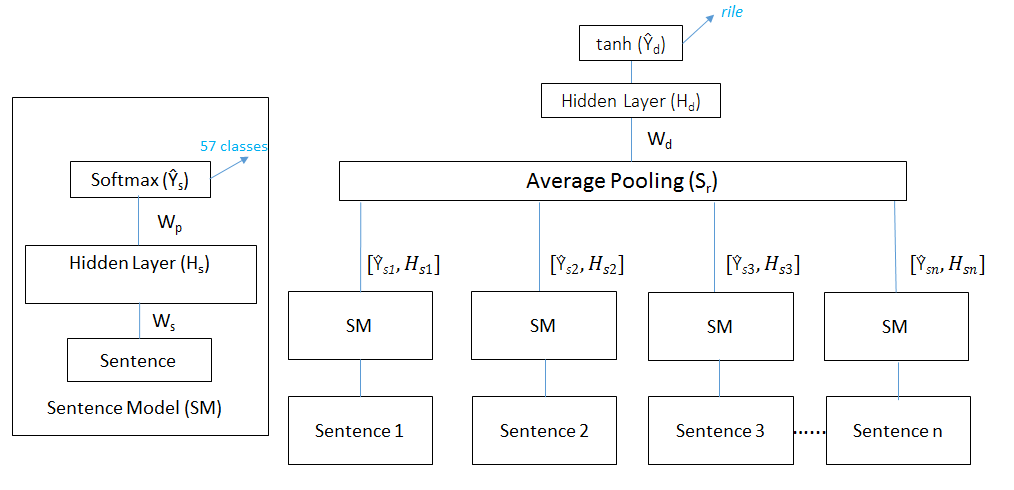
\includegraphics[height=6.5cm, scale=0.8]{JointModel11.png}
\caption{Hierarchical Neural Network for Joint Sentence-Document Analysis. Optimal model parameters we found --- $\norm{H_{s}}$ = 300, $\norm{H_{d}}$ = 10}
 \label{fig:HNN}
 \end{figure*}

\subsection{Sentence Level Model}
We represent each sentence using average embedding of its constituent words.
\[ s_{i} = \frac{1}{|s_{i}|}\sum_{w \in s_{i}} emb(w) \]
The average embedding representation is given as input to hidden layer with rectified linear activation units (ReLU) to get the hidden representation, which is defined as 
\[H_{s_{i}}= \max(0,a)\] where, $a = W_{s}^{T}s_{i}$. Finally, the predictions are obtained using a softmax layer, which takes the hidden representation as input and gives probability of 57 classes as output.
\[ \hat{Y}_{s_{ik}} = \frac{e^{H_{s_{i}}^T w_{pk}}}{\sum_{j=1}^{K}{e^{H_{s_{i}}^T w_{pj}}}}\]
We use cross-entropy loss function for sentence level model. For sentences in $D_{s}$, with ground truth labels $Y_{s}$ (one-of-K encoding), the loss function is given as follows

\[ L_{S}(D_{s},Y_{s})=-\frac{1}{\sum_{i=1}^{D_{s}}l_{d_{i}}}\sum_{i=1}^{D_{s}}\sum_{j=1}^{l_{d_{i}}}\sum_{k=1}^{K} Y_{s_{ijk}} \ln \hat{Y}_{s_{ijk}}  \]

\subsection{Joint Sentence-Document Model}
Using the Hierarchical Neural Network, we model both sentence level classification and document level regression tasks together. In the combined model, we use unrolled (time-distributed\footnote{\url{https://keras.io/layers/wrappers/\#timedistributed}}) neural network model for the sentences in a manifesto. Here, the model minimizes cross-entropy loss for sentences over each temporal layer ($1$ to $n$). We use average-pooling to create document representation with individual sentence representations. We concatenate hidden representation ($H_{s}$) and predicted output distribution ($\hat{Y}_{s}$) of sentences before average-pooling\footnote{We observed that the concatenated representation performed better than using either hidden representation or output distribution}.

\[ S_{r} = \frac{1}{|l_{d_{i}}|}\sum_{s \in d_{i}} [\hat{Y}_{s}, H_{s}] \]

\textit{rile} varies from -100 to +100, we scale it to a range between -1 and +1. So, we use tanh layer finally to get regressed output with $z = H_{d} = ReLU(W_{d}^{T}S_{r})$ as input.

\[ \hat{Y}_{d} = tanh(z) = \frac{e^z - e^{-z}}{e^z + e^{-z}} \]

Since it is a regression task, we minimize mean-squared error loss function between the predicted $\hat{Y}_{d}$ and actual rile scores $Y_{d}$.

\[ L_{d}(\hat{Y}_{d}, Y_{d}) = \frac{1}{|D|} \sum_{d=1}^{D} (\hat{Y}_{d} - Y_{d})^2 \]

Overall, the combined loss function for the joint model is 

\begin{equation}
 L_{s}(D_{s},Y_{s}) + L_{d}(\hat{Y}_{d}, Y_{d}) 
\end{equation}
%\footnote{http://128.2.220.95/multilingual}

We evaluate both cascaded and joint training for this objective function. We use Adam optimizer\footnote{\url{https://keras.io/optimizers/\#adam}} for parameter estimation. 
\begin{itemize}
\item{Cascaded Training:} In this approach sentence level model is trained using $D_{s}$, to minimize $L_{s}(D_{s},Y_{s})$, and the pre-trained model is used to obtain document level representation $S_{r}$ for all the manifestos in training set, $D$. Then the document level regression task is trained to minimize $L_{d}(\hat{Y}_{d}, Y_{d})$. Here, the sentence level model parameters are fixed when the document level regression model is trained using $S_{r}$.

\item{Joint Training:} Here the entire network is updated by minimizing the joint loss function (2). The sentence level model uses both labeled and unlabeled data, where the updates using unlabeled data is influenced by document level objective.
\end{itemize}

%again, the sentence level model is trained using $D_{s}$, to minimize $L_{d}(D_{s},Y_{g})$. Then

The proposed architecture evaluates the effectiveness of posing sentence-level topic classification task as a precursor to solve document level \textit{rile} prediction, rather than learning a model directly. Secondly, we also study the utility of having more document level annotations --- one-dimensional scores on the left-right spectrum, compared to sentence level annotations, especially for sentence level thematic classification task. Finally, the document level \textit{rile} score estimation can be replaced with any other task in the proposed architecture --- expert survey or voter survey scores.

\section{Experimental Results}
As mentioned earlier, we use manifestos collected and annotated by political scientists at CMP. In this work, we used digitized manifestos from 13 countries, 948 in total which are written in 6 different languages --- Danish (Denmark), English (Australia, Ireland, New Zealand, South Africa, United Kingdom, United States), Finnish (Finland), French (France), German (Austria, Germany, Switzerland) and Italian (Italy). Out of the 948 manifestos, 235 are annotated with sentence level labels (Figure \ref{fig:CMP}). We have \textit{rile} scores for all the 948 manifestos. Statistics about number of annotated documents and sentences with fine-grained labels (from Figure \ref{fig:CMP}) across languages is given below.
 \begin{table}[!ht]
  \centering
  \begin{tabular}{ c c c }
  \toprule
    Lang. & \# Docs (Antd.) & \# Sents (Antd.)\\
    \midrule
    da  & 175 (36)  &  32161 (8762)	\\
    en   &  312 (94)& 227769 (73682) 	 \\    	
    fi  &  97 (16) &  18717 (8503) \\
    fr    & 53 (10) & 24596 (5559)\\
    de    & 216 (65) & 146605 (79507) \\
    it    & 95 (14)  & 40010 (4918)\\
\midrule
 Total    & 948 (235)  & 489858 (180931)\\
    \bottomrule

  \end{tabular}
  \caption{Statistics of dataset, `Antd.' refers to annotated. \textit{da - Danish, en - English, fi - Finnish, fr - French, de - German, it - Italian}}
  \label{tab:al}
\end{table}

We use off-the-shelf multi-lingual word embeddings\footnote{\url{http://128.2.220.95/multilingual}} to represent words. We chose embeddings trained using translation invariance approach \cite{ammar2016massively}, with size 512 for our work, since we found it empirically better compared to other approaches. As mentioned in Section 4.1, we use average embedding as sentence representation. Following are the sentence classification baseline techniques that we compare our proposed approach against.

\begin{description}
\item{\textit{Bag of words:}} We use TF-IDF representation for sentences and build a model for each language separately. We use Logistic Regression classifier, which is the state-of-art approach for fine-grained (57 classes) manifesto sentence classification \cite{biessmann2016automating}. We refer to this approach as \textit{LR}. We also use Neural Network classifier, which we refer as \textit{NN}.

\item{\textit{Language-wise average embedding:}} We build a Neural Network (LW-NN) classifier per language, with average neural embedding as sentence representation.

\item{\textit{Convolutional Neural Network:}} CNN was shown to be effective for cross-lingual manifesto text coarse-level (7 major domains as shown in Figure \ref{fig:CMP}) topic classification \cite{W17-2906}. So, we evaluate CNN with a similar architecture --- single convolution (32 filters with window size 3), single max pooling layer and finally a softmax layer. We use neural embeddings to represent words. Similar to \cite{W17-2906} we combined training instances across all the languages.
\end{description}

For document level regression task, following are the baseline approaches. Note that we use \textit{tanh} output for all the models, since the range of re-scaled \textit{rile} is from -1 to +1.

% with \textit{tanh} output.
\begin{description}
\item{\textit{Bag of words:}} We use TF-IDF representation for documents and build a regression model for each country and language separately. We use Linear Regression; referred to as \textit{LR-CTR} and \textit{LR-Lang} which are models built per country and language respectively. Since language-wise model performed better than country-wise model, we also build a Neural Network model (to capture non-linear patterns) for each language, \textit{NN-Lang}.

\item{\textit{Average embedding (\textit{Doc-Avg}):}} We use average embedding of words in the document as representation, with Neural Network model.

\item{\textit{Bag-of-Centroids ($BoC$):}} Here the word embeddings are clustered into $K$ different clusters using K-Means clustering algorithm, and  words in each document are assigned to clusters based on its euclidean-distance ($dist$) to cluster-centroids ($C$). 
\[ cluster (word) = \argmin_k dist(C_{k}, word) \]
Finally, each document is represented by the distribution of words mapped to different clusters (1 X $K$ vector). We use a Neural Network regression model with bag-of-centroids representation. Results with $K$=1000, which performed best is given in Table 3.

\item{Sentence level model and RILE formulation \textit{(SRILE)}:} Here the predictions of sentence level model in the cascaded approach are used directly with \textit{rile} formulation (equation (1)) to derive $rile$ score for manifestos.

\item{\textit{Cross-lingual scaling ($CLS$):}} This is a recent unsupervised approach for multi-lingual political speech text positioning task \cite{EACL}. Authors use average word-embeddings weighed by TF-IDF score to represent documents\footnote{We use this aggregate representation since it was shown to be better than word alignment and scoring approach \cite{EACL}}. Then a graph is constructed using pair-wise distance of documents. Given two pivots texts for extreme left and right positions [-1, +1], label propagation approach is used to quantify other documents in the graph.
\end{description}

 \begin{table*}[!htb]
  \centering
  \begin{tabular}{ c c c c c c c}
  \toprule
    Lang. & LR & NN & LW-NN & CNN & Cas-S & JT-S\\
    \midrule
    da  & 	0.29 & \textbf{0.36} & 0.24 & 0.30 & 0.28 & 0.30\\
    en   &  0.24 & 0.29 & \textbf{0.43} & 0.40 & 0.42 & 0.41\\    	
    fi  &   0.21 & 0.23 & 0.26 & \textbf{0.30} & 0.27 & 0.26\\
    fr    & 0.28 & 0.28 & 0.24 & 0.36 & 0.37 & \textbf{0.38} \\
    de    &  0.20 & 0.23 & 0.31 & 0.31 & 0.31 & \textbf{0.33}\\
    it    & 0.14 & 0.22 & 0.25 & 0.30 & \textbf{0.32} & 0.26\\
\midrule
Avg.    & 0.22 & 0.26 & 0.35 & 0.34 & \textbf{0.36} & 0.35\\
    \bottomrule

  \end{tabular}
  \caption{Micro-Averaged F-measure. Best scores are given in bold under each language setting}
  \label{tab:al}
\end{table*}

We compute average performance with 80-20\% train-test ratio across 10 runs with random split, where the 80\% split also contains sentence level annotated documents proportionally.  We compute average F-score\footnote{Harmonic mean of precision and recall, \url{https://en.wikipedia.org/wiki/F1_score}} to evaluate sentence classification performance. Sentence classification performance is given in Table 2. The proposed approach trained using \textit{cascaded training} is referred to \textit{Cas-S}. Note that in \textit{cascaded training}, sentence and document level models are trained separately in a cascaded fashion. Joint-training results where the sentence model is trained in a semi-supervised way together with document level regression task is referred to as \textit{JT-S}.  We observed that \textit{JT-S} has a comparable performance with \textit{Cas-S}. Also \textit{CNN}, \textit{Cas-S} and \textit{JT-S} use combined training instances across languages compared to other approaches. Hence other than en and de which have sufficient labeled data, models that use combined training data perform better. Secondly, in the mono-lingual setting, using word embeddings provides better performance compared to bag-of-words for en, fi, de and it.

 \begin{table}[H]
  \centering
  \begin{tabular}{ c c c }
  \toprule
    Approach & MSE & $r$\\
    \midrule
    LR-CTR  & 	0.874 & 0.18 \\
    LR-Lang   &  0.684 & 0.24\\    	
    NN-Lang  &   0.054 & 0.23\\
    Doc-Avg    & 0.057 & 0.14\\
    BoC    &  0.052 & 0.33\\
    SRILE   & 0.060 & 0.35\\
    %CLS   & 0.815 & 0.24\\
    CLS   & -- & 0.24\\
    Cas-D  &  0.051 & 0.41 \\
    JT-D &  \textbf{0.044} & \textbf{0.47} \\
    \bottomrule
  \end{tabular}
  \caption{$rile$ score prediction performance. Best scores are given in bold. \begin{small}CLS assigns -1 and +1 for extreme manifestos and propagates the values on a graph. Since they solve it as a classification problem, MSE is not applicable\end{small}}
  \label{tab:al}
\end{table}

\textit{rile} score regression performance results are given in Table 3.  We evaluate document level performance using mean-squared-error (MSE) and Pearson correlation ($r$).
The proposed approach using cascaded training with fixed sentence model parameters is referred to as \textit{Cas-D} and jointly trained model is referred to as \textit{JT-D}. Overall we the jointly trained model performs best for document level task, with a comparable performance at sentence level.

% \subsection{Joint Training}
% Here we provide results for the joint model, where the sentence model is trained in a semi-supervised way together with document level regression task. We observed that the jointly trained model did not perform better than cascaded model fine-tuned for document level task.

\subsection{Quantity of Annotation}
We measure the importance of annotated text at sentence and document level for \textit{rile} score regression task. We vary the percentage of labeled data, while keeping the test sample size at 20\% as before. In the first setting, we keep the training ratio of documents at 80\%, within that 80\% we increase the proportion of documents with sentence level annotations --- from 0 (document average embedding setting, \textit{Doc-Avg}) to 80\%. Results are given in Figure \ref{fig:sentl}. Similarly, in the other setting, we keep the training set with 80\% sentence level annotated documents (which is $\sim$20\% of the total data), and add documents (with only \textit{rile} score), increasing the training set from 20 to 80\%. Results of this study are given in Figure \ref{fig:docl}. We observe that, jointly-trained model uses sentence level annotations more effectively than cascaded approach (Figure \ref{fig:sentl}) --- even with less sentence level annotations. Also, with less document level signal (upto 40\%) for training, both the approaches perform similarly. As the training ratio increases, joint-training leverages both sentence and document level signals effectively.

\begin{figure}[!ht]
\centering
  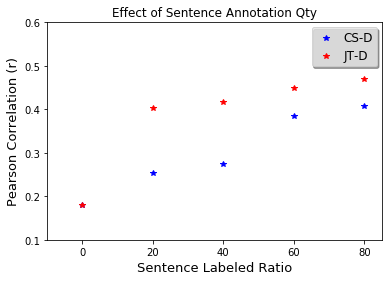
\includegraphics[width=0.9\linewidth]{Plot1.png}
  \caption{Fixing 80\% training documents with rile score, ratio of documents with sentence level annotations is varied}
  \label{fig:sentl}
\end{figure}

\begin{figure}[!ht]
\centering
  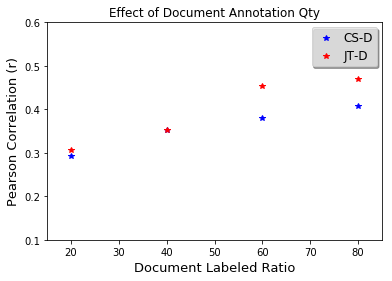
\includegraphics[width=0.9\linewidth]{Plot2.png}
  \caption{Fixing 80\% training documents with sentence level annotations, ratio of documents with rile score is varied}
 \label{fig:docl}
 \end{figure}
 
\subsection{Use of Country Information}
Since the definition of left-right varies between countries, we study the influence of \textit{country} information in the proposed model (\textit{JT-D}) with \textit{joint-training}. We use two ways to incorporate country information: (a) \textit{stack} --- one-hot encoding (13 countries, 1 X 13 vector) of each manifesto's \textit{country} is concatenated with hidden representation of the document ($S_{r}$ in Figure \ref{fig:HNN}) (b) \textit{non-linear stack} --- one-hot-encoded country vector is passed through a hidden layer with \textit{tanh} non-linear activation and concatenated with $S_{r}$. With both the models we observed mild improvement in correlation (given in Table \ref{tab:al}).

 \begin{table}[H]
  \centering
  \begin{tabular}{ c c c }
  \toprule
    Approach & MSE & $r$\\
    \midrule
    stack &  0.045 (0.001 $\downarrow$) & 0.49 (0.02 $\uparrow$) \\
    non-linear stack &  0.048 (0.004 $\downarrow$) & 0.48 (0.01 $\uparrow$) \\
    \bottomrule
  \end{tabular}
  \caption{$rile$ score performance with country information. Difference compared to \textit{JT-D} is given within paranthesis. $\uparrow$ -- improvement, $\downarrow$ -- decrease in performance}
  \label{tab:al}
\end{table}

\section{Conclusion and Future Work}
In this work we evaluated the utility of a joint sentence-document model for sentence level thematic classification and document level \textit{rile} score regression tasks. Our observations are as follows: (a) joint model performs better than state-of-art approaches (b) joint-training leverages sentence level annotations more effectively than cascaded approach for \textit{rile} score regression task.
There are many extensions possible to the current work. First is to handle class imbalance in the dataset with a cost-sensitive objective function. Secondly, CNN gave a comparable performance with Multi-layer Perceptron (NN), which motivates the need to evaluate an end-end sequential architecture. We used off-the-shelf embeddings, which leads to out-of-vocabulary scenarios. It could be beneficial to  adapt word-embeddings with manifesto corpus. Finally, background information such as country can be leveraged more effectively.

\begin{figure*}[!ht]
\centering
\begin{subfigure}{.45\textwidth}
  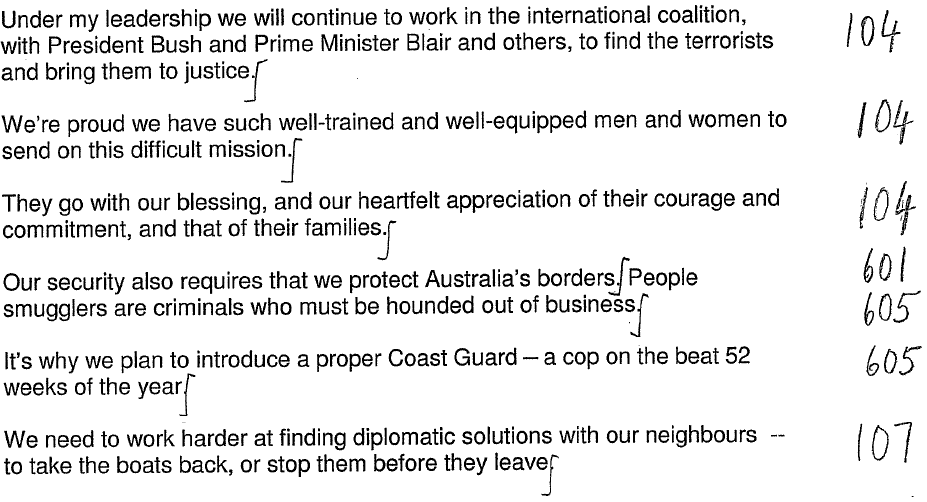
\includegraphics[width=1\linewidth]{Aus_Labor.png}
  \caption{Australian Labor Party, 2001}
  \label{fig:sub1}
\end{subfigure}%
\begin{subfigure}{.55\textwidth}
  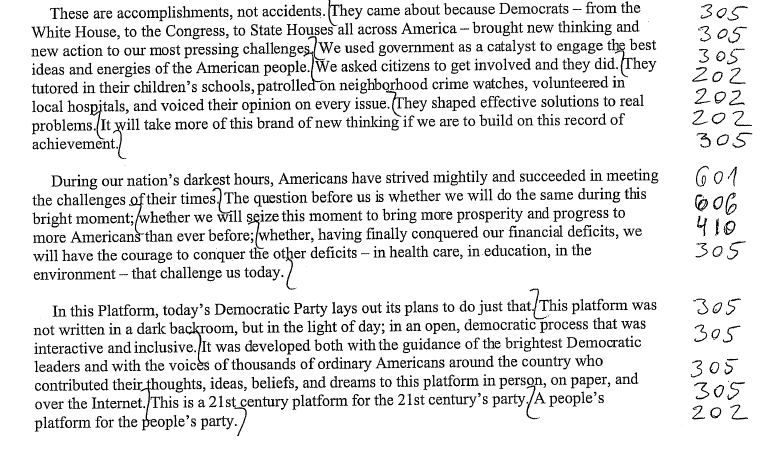
\includegraphics[width=1.1\linewidth]{US_Democrats.png}
  \caption{Democratic Party of USA, 2000}
  \label{fig:sub2}
 \end{subfigure}
 \caption{Sample Manifestos --- $\int$ denotes sentence segment}
 \end{figure*}
 
\begin{figure*}[!ht]
\centering
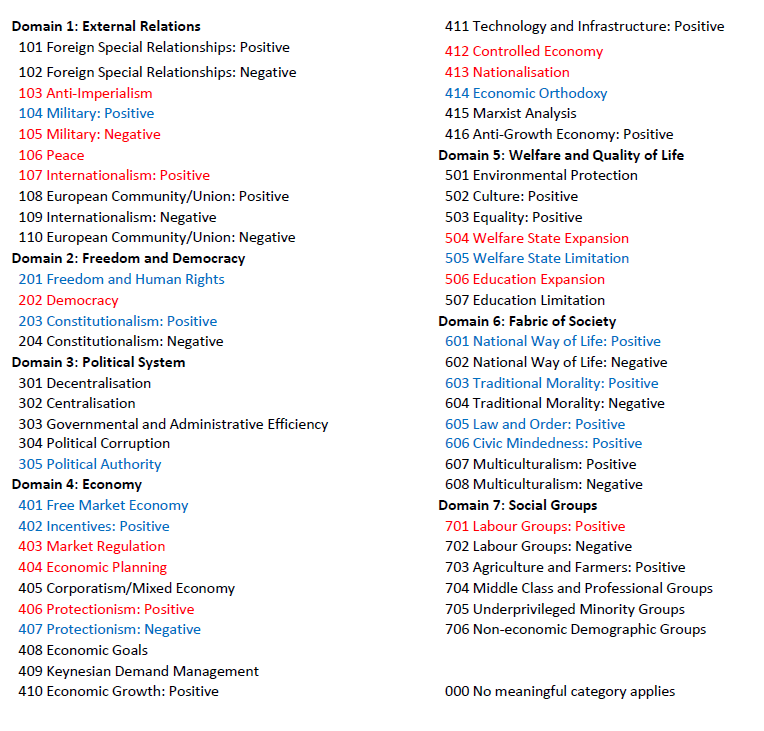
\includegraphics[width=1\linewidth]{CMP_Coding_1.png}
\caption{\textit{Left} topics are given in red, \textit{right} topics are given in blue and the rest are given in black}
\label{fig:CMP}
\end{figure*}

\bibliography{acl2017}
\bibliographystyle{acl_natbib}

%\section{Appendix}



% \begin{figure*}[ht]
% \centering
% \begin{subfigure}{.45\textwidth}
%   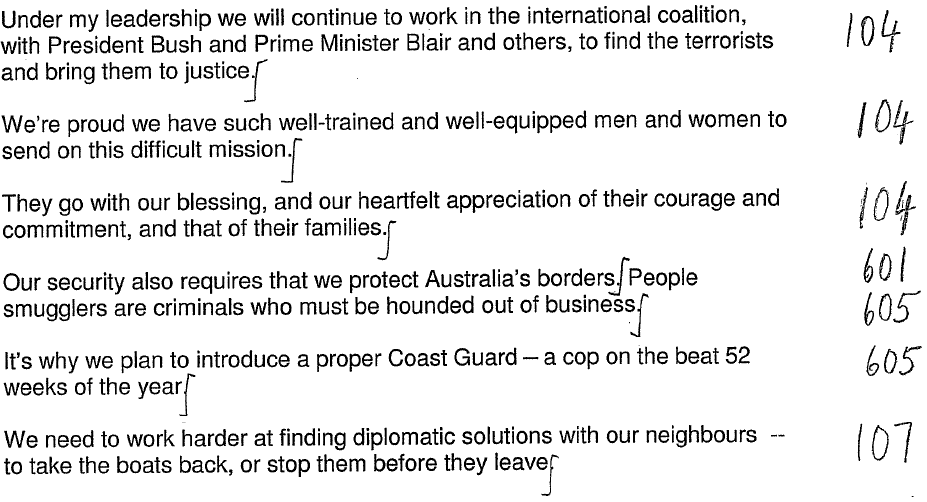
\includegraphics[width=1\linewidth]{Aus_Labor.png}
%   \caption{Australian Labor Party, 2001}
%   \label{fig:sub1}
% \end{subfigure}%
% \begin{subfigure}{.55\textwidth}
%   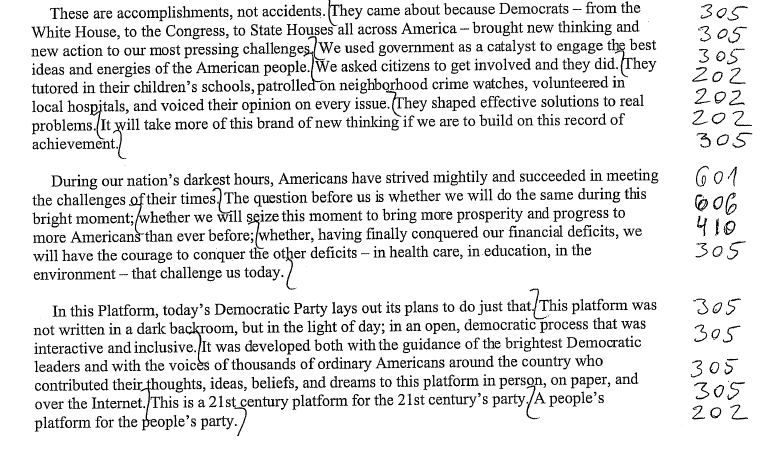
\includegraphics[width=1\linewidth]{US_Democrats.png}
%   \caption{Democratic Party of USA, 2000}
%   \label{fig:sub2}
%  \end{subfigure}
%   \begin{subfigure}{.6\textwidth}
%   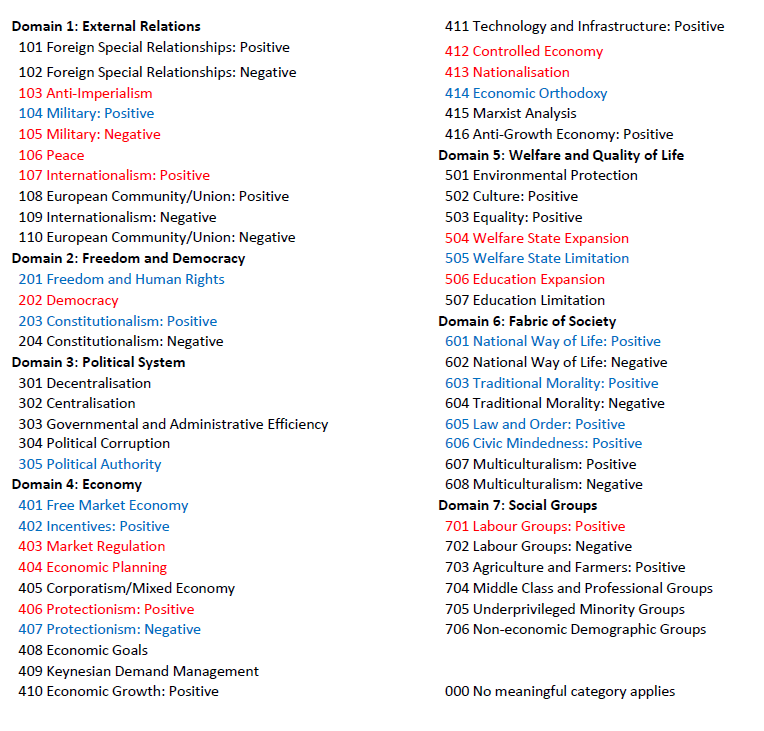
\includegraphics[width=1.3\linewidth]{CMP_Coding_1.png}
%   \caption{\textit{Left} topics are given in red, \textit{right} topics are given in blue and the rest are given in black}
%   \end{subfigure}
% \caption{Sample Manifestos (a and b) and CMP coding scheme (c)}
% \label{fig:test}
%  \end{figure*}
 
\end{document}
